This is reference manual for the GuardTime client SDK. The SDK offers functions and examples useful for developers who want to integrate GuardTime timestamps into their own applications.

Disclaimer: This is the first public release of the SDK. We expect to deliver updates based on feedback from the first users and cannot guarantee that the updated versions will maintain interface compatibility with the current release.

\subsection*{Timestamps}

A timestamp contains the information to certify that some data existed in a given form at some given time in the past. Timestamps are normally issued by trusted third parties called Timestamping Authorities (TSAs). The main innovation in GuardTime timestamps is that the amount of trust in the TSA required from the customers is significantly reduced compared to the more traditional approaches.

The two main operations on timestamps are generation and verification. Generation of a timestamp involves cryptographically binding the data whose integrity is to be protected to the time value from a reliable source in a way that neither the data nor the time value could later be changed undetectably. Verification means checking that the binding is still intact.

To get a timestamp from a GuardTime timestamping service, the client application computes a hash value of the data to be timestamped and submits the hash value to the timestamping service. The service returns a timestamp binding the hash value to the current time. The interaction follows the standard timestamping protocol defined in the RFC 3161.

A hash value is like a digital fingerprint of the data. Given both the original data and the hash value, it is easy to verify that they match. Yet it is impossible to recover the original data from the hash value, much like it is not possible to reconstruct a person from his/her fingerprint. So, even confidential data can be timestamped without any fear of disclosure. It is also quite impossible to create two different documents having the same fingerprint.

Every month, GuardTime creates an Integrity Code and publishes it in several newspapers across the world. The Integrity Code is a summary of all timestamps issued by the GuardTime timestamping services. Any timestamp issued prior to the creation of the Integrity Code can be traced to it to unambiguously prove the timestamp's age and integrity.

The proof connecting the timestamp to the Integrity Code can be inserted back into the timestamp itself in a process we call extending the timestamp. An extended timestamp is completely independent of GuardTime. Only the original data, the timestamp and any copy of the newspaper where the Integrity Code is published will be necessary to prove the intgerity and the age of the document.

Until the Integrity Code is generated, the timestamps are protected by GuardTime's digital signature. Digitally signing timestamps is the most common mode of operation of TSAs. The independent proof of authenticity based on publically available data is what makes GuardTime's solution unique.

For convenience, GuardTime publishes an electronic archive containing all Integrity Codes since the launch of the service and all valid signing keys. This electronic archive can be used to automate mass verification of thousands of timestamps (whether extended or not) per second in a large archive.

 
\begin{DoxyImageNoCaption}
  \mbox{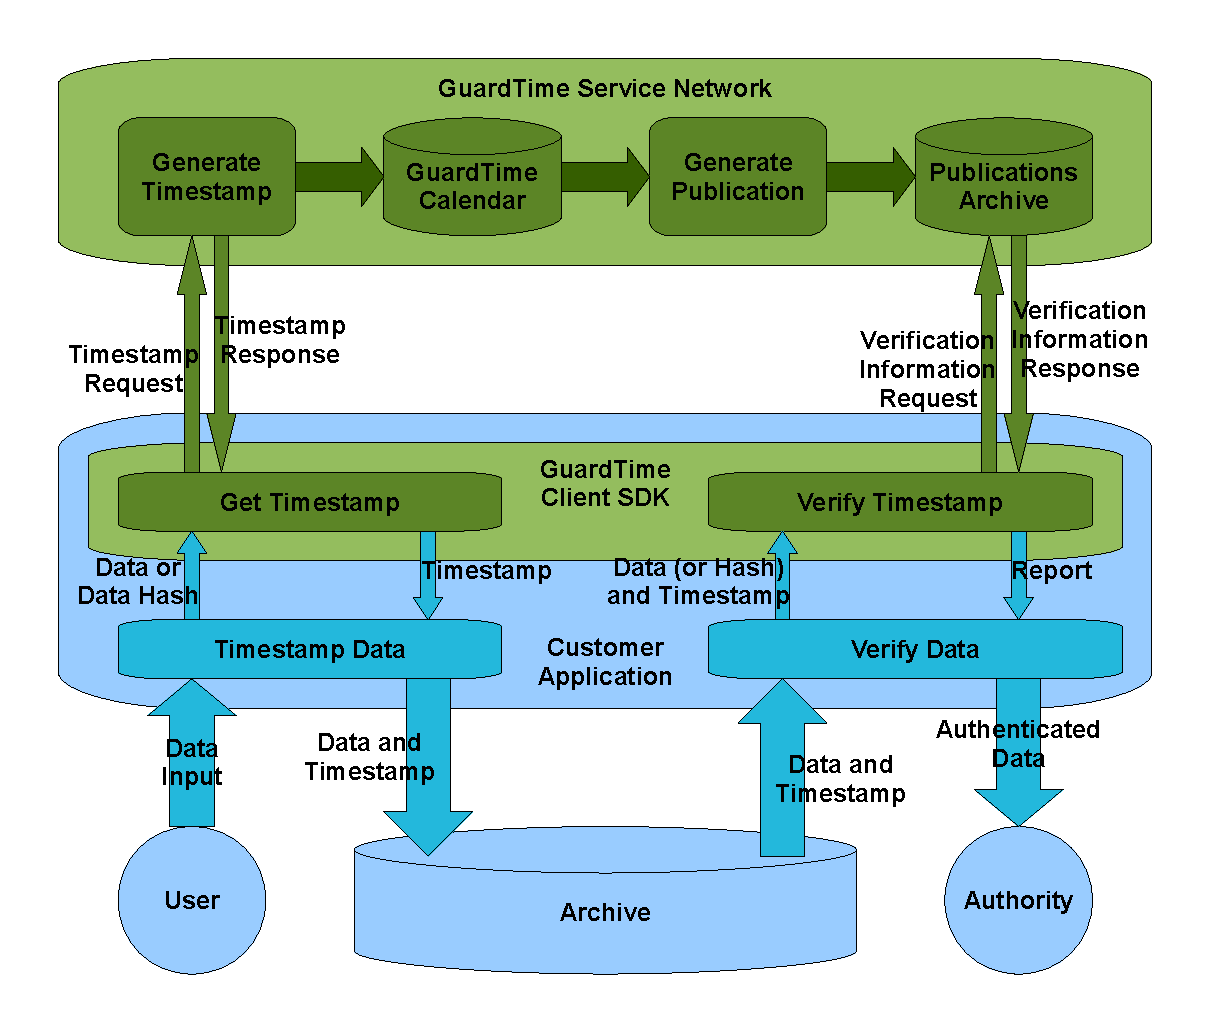
\includegraphics[width=15cm]{TspOverview}}
\end{DoxyImageNoCaption}


\subsection*{Structure}

For manageability, the GuardTime client SDK is split into several layers.

{\bfseries The Base API}

The base API deals with the low-\/level details of handling the timestamps. The public interface of this layer is defined in the file {\ttfamily \hyperlink{gt__base_8h}{gt\_\-base.h}} and the implementation is provided in the library {\ttfamily libgtbase}.

The functions in this layer cover the follwoing functional areas:
\begin{DoxyItemize}
\item the \hyperlink{group__timestamps}{Timestamps} section describes the functions dealing with creation, encoding and decoding of timestamp objects;
\item the \hyperlink{group__publications}{Publications} section describes the functions for handling the electronic archives of Integrity Codes;
\item the \hyperlink{group__verification}{Verification} section describes the functions for verifying the validity of timestamps;
\item the \hyperlink{group__common}{Common} section collects various helper functions, such as for data hashing and error handling.
\end{DoxyItemize}

The cryptographic functions in the base API rely on the OpenSSL library, which has to be available to your application. See the documentation for the header file for more details on this.

{\bfseries The HTTP Transport}

This module deals with communicating to the GuardTime network over the HTTP protocol. The public interface of this layer is defined in the file {\ttfamily \hyperlink{gt__http_8h}{gt\_\-http.h}} and the implementation is provided in the library {\ttfamily libgthttp}.

Detailed documentation for this layer is available in the \hyperlink{group__http}{HTTP transport} section.

For actual network transport on Linux, this module relies on the cURL library, which has to be available to your application. On Windows, the module relies on WinINet which comes standard on all supported versions of Windows. See the documentation for the header file for more details on this.

The HTTP module also uses the base API for handling the timestamps.

{\bfseries The PNG Integration}

This module deals with seamless embedding of GuardTime timestamps into PNG image files. The public interface of this layer is defined in the file {\ttfamily \hyperlink{gt__png_8h}{gt\_\-png.h}} and the implementation is provided in the library {\ttfamily libgtpng}.

Detailed documentation for this module is available in the \hyperlink{group__png}{PNG integration} section.

This module does not have any external dependencies, but it does rely on the base API and the HTTP module.

We expect to provide similar modules for several other file formats in the next release of the GuardTime client SDK.

\subsection*{Examples}

The SDK includes simple command line utilities for timestamping arbitrary files and verifying the timestamps.

{\bfseries Creating a timestamp}

The timestamping utility is located in the file {\ttfamily src/http/http\_\-create.c} within the SDK source code archive.

To compile the example under Linux, use a command along the lines of 
\begin{DoxyCode}
        gcc http_create.c -o http_create -I/usr/local/gt/include \
        -L/usr/local/gt/lib -L/usr/local/curl/lib -L/usr/local/ssl/lib \
        -lgthttp -lgtbase -lcurl -lcrypto -lrt
\end{DoxyCode}
 (either with the backslashes or all on a single line) replacing {\ttfamily /usr/local/gt}, {\ttfamily /usr/local/curl} and {\ttfamily /usr/local/ssl} with the directories where you unpacked the GuardTime, cURL and OpenSSL libraries (you can skip the {\ttfamily /I} and {\ttfamily /L} options if you installed everything in standard system locations).

To compile the example under Windows, use a command along the lines of 
\begin{DoxyCode}
        cl.exe http_create.c /MT /I C:\gt\include
        /link /libpath:C:\gt\lib /libpath:C:\openssl\lib
        libgthttpMT.lib libgtbaseMT.lib libeay32MT.lib wininet.lib
        wsock32.lib wldap32.lib winmm.lib user32.lib gdi32.lib advapi32.lib
\end{DoxyCode}
 (all on a single line) replacing {\ttfamily C:$\backslash$gt} and {\ttfamily C:$\backslash$openssl} with the directories where you unpacked the GuardTime and OpenSSL libraries.

To run the compiled example, use a command along the lines of 
\begin{DoxyCode}
        http_create data_in_file timestamp_out_file stamper_url
\end{DoxyCode}
 where the data is to be read from the file {\ttfamily data\_\-in\_\-file}, the timestamp is to be written to the file {\ttfamily timestamp\_\-out\_\-file} and the timestamping service is located at the URL {\ttfamily stamper\_\-url}.

The core of the example is as follows: 
\begin{DoxyCode}
        // Error handling omitted for brevity
        // See the actual source code for full details

        // Hash the data file
        GT_hashFile(in_file, GT_HASHALG_DEFAULT, &data_hash);

        // Get the timestamp
        GTHTTP_createTimestampHash(data_hash, tsa_url, &timestamp);

        // Encode the timestamp
        GTTimestamp_getDEREncoded(timestamp, &der, &der_len);

        // Save the DER-encoded timestamp to a file
        GT_saveFile(out_file, der, der_len);
\end{DoxyCode}


{\bfseries Verifying a timestamp}

The timestamp verification utility is located in the file {\ttfamily src/http/http\_\-verify.c} within the SDK source code archive.

To compile the example under Linux, use a command along the lines of 
\begin{DoxyCode}
        gcc http_verify.c -o http_verify -I/usr/local/gt/include \
        -L/usr/local/gt/lib -L/usr/local/curl/lib -L/usr/local/ssl/lib \
        -lgthttp -lgtbase -lcurl -lcrypto -lrt
\end{DoxyCode}
 (either with the backslashes or all on a single line) replacing {\ttfamily /usr/local/gt}, {\ttfamily /usr/local/curl} and {\ttfamily /usr/local/ssl} with the directories where you unpacked the GuardTime, cURL and OpenSSL libraries (you can skip the {\ttfamily /I} and {\ttfamily /L} option if you installed everything in standard system locations).

To compile the example under Windows, use a command along the lines of 
\begin{DoxyCode}
        cl.exe http_verify.c /MT /I C:\gt\include
        /link /libpath:C:\gt\lib /libpath:C:\openssl\lib
        libgthttpMT.lib libgtbaseMT.lib libeay32MT.lib wininet.lib
        wsock32.lib wldap32.lib winmm.lib user32.lib gdi32.lib advapi32.lib
\end{DoxyCode}
 (all on a single line) replacing {\ttfamily C:$\backslash$gt} and {\ttfamily C:$\backslash$openssl} with the directories where you unpacked the GuardTime and OpenSSL libraries.

To run the compiled example, use a command along the lines of 
\begin{DoxyCode}
        http_verify timestamp_in_file data_in_file publications_url verifier_url
\end{DoxyCode}
 where the timestamp is to be read from the file {\ttfamily timestamp\_\-in\_\-file}, the data is to be read from the file {\ttfamily data\_\-in\_\-file}, the publications list is to be retrieved from the URL {\ttfamily publications\_\-url} and the online verifying service is located at the URL {\ttfamily verifier\_\-url} (the last one is optional, specify {\ttfamily -\/} instead of the URL for offline verification).

The core of the example is as follows: 
\begin{DoxyCode}
        // Error handling omitted for brevity
        // See the actual source code for full details

        // Read the timestamp file
        GT_loadFile(timestamp_file, &stamp_der, &stamp_der_len);

        // Decode the timestamp
        GTTimestamp_DERDecode(stamp_der, stamp_der_len, &timestamp);

        // Hash the data file
        GTTimestamp_getAlgorithm(timestamp, &hash_algo);
        GT_hashFile(data_file, hash_algo, &data_hash);

        // Verify the timestamp
        GTHTTP_verifyTimestampHash(timestamp, data_hash,
                verifier_url, NULL, NULL, publications_url, 0, &ver);

        // Display the results
        GTVerificationInfo_print(stderr, 0, ver);
        if (ver->verification_errors == GT_NO_FAILURES) {
                printf("Verification succeeded!\n");
        }
\end{DoxyCode}


\subsection*{License}

Copyright 2008-\/2010 GuardTime AS

Licensed under the Apache License, Version 2.0 (the \char`\"{}License\char`\"{}); you may not use this file except in compliance with the License. You may obtain a copy of the License at \href{http://www.apache.org/licenses/LICENSE-2.0}{\tt http://www.apache.org/licenses/LICENSE-\/2.0}.

Unless required by applicable law or agreed to in writing, software distributed under the License is distributed on an \char`\"{}AS IS\char`\"{} BASIS, WITHOUT WARRANTIES OR CONDITIONS OF ANY KIND, either express or implied. See the License for the specific language governing permissions and limitations under the License.

\subsection*{Acknowledgements}

This product includes software developed by the OpenSSL Project for use in the OpenSSL Toolkit (\href{http://www.openssl.org/}{\tt www.openssl.org}).

This product includes cryptographic software written by Eric Young (\href{mailto:eay@cryptsoft.com}{\tt eay@cryptsoft.com}). This product includes software written by Tim Hudson (\href{mailto:tjh@cryptsoft.com}{\tt tjh@cryptsoft.com}).

This product includes networking software developed by the cURL Project (\href{http://curl.haxx.se/}{\tt curl.haxx.se}). 